%\documentclass[12pt]{article}
%\usepackage[a4paper, margin=1in]{geometry} 
%\usepackage{graphicx} 
%\usepackage{hyperref}
%\usepackage{float}
%\usepackage{multicol}
%\usepackage{multirow}
%\usepackage{amsmath}
%\usepackage[font=small, labelfont=bf]{caption}
%
%\begin{document}

%
% Distance-based methods
%
\subsection{Distance-based methods}
PGMA (pair-group method using arithmetic mean) and neighbor-joining are two popular distance-based methods to reconstruct a phylogenetic tree.

%
%  UPGMA
%
\subsubsection*{UPGMA}
UPGMA is an unweighted version of PGMA. It requires the evolutionary rate should be constant (ultrametric). Pairwise distances need to be pre-calculated, for instance, by DP.

\begin{itemize}
\item $w$: A new node
\item $u$, $\upsilon$: Child nodes of $w$
\item $m_{A}$ The number of original sequences in subtree $A$
\item $D_{A,B}$: Distance between sequences/subtrees $A$ and $B$
\end{itemize}

\[
D_{w,x}=\dfrac{m_{u}D_{u,x} + m_{\upsilon}D_{\upsilon,x}}{m_{u} + m_{\upsilon}}
\]

%
% Example of UPGMA
%
\subsubsection*{Example of UPGMA}
Reconstruct a phylogenetic tree from the pre-calculated distances below.

\begin{table}[H]
\centering
\begin{tabular}{|l|l|l|l|}
\hline
  & B & C & D \\ \hline
A & 4 & 2 & 5 \\ \hline
B &   & 4 & 8 \\ \hline
C &   &   & 5 \\ \hline
\end{tabular}
\end{table}

\noindent
\textbf{Step 1a}.
Find a pair with the closest distance
\begin{figure}[H]
  \centering
      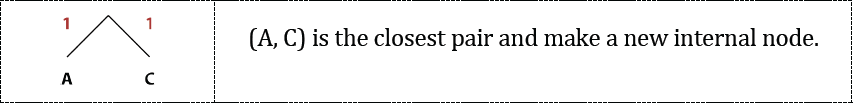
\includegraphics[width=0.9 \textwidth]{fig09/upgma_1.png}
\end{figure}

\noindent
\textbf{Step 1b}.
Recalculate the distances
\[
d_{B,(AC)}=\dfrac{d_{B,A} + d_{B,C}}{2} = 4, \quad d_{D,(AC)}=\dfrac{d_{D,A} + d_{D,C}}{2} = 5
\]

\noindent
\textbf{Step 1c}.
Update the distance matrix with a new node (AC)
\begin{table}[H]
\centering
\begin{tabular}{|l|l|l|}
\hline
     & B & D \\ \hline
(AC) & 4 & 5 \\ \hline
B    &   & 8 \\ \hline
\end{tabular}
\end{table}

\noindent
\textbf{Step 2a}.
Find a pair with the closest distance
\begin{figure}[H]
  \centering
      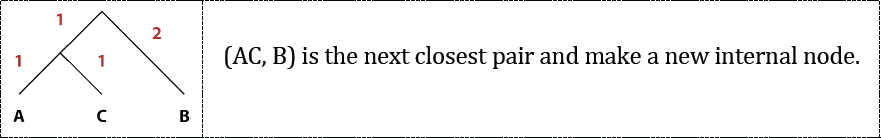
\includegraphics[width=0.9 \textwidth]{fig09/upgma_2.png}
\end{figure}

\noindent
\textbf{Step 2b}.
Recalculate the distance
\[
d_{((AC)B),D}=\dfrac{2 \times d_{(AC),D} + d_{B,D}}{3} = 6
\]

\noindent
\textbf{Step 2c}.
Update the distance matrix with a new node ((AC)B)
\begin{table}[H]
\centering
\begin{tabular}{|l|l|}
\hline
        & D \\ \hline
((AC)B) & 6 \\ \hline
\end{tabular}
\end{table}

\noindent
\textbf{Step 3}.
Complete the tree
\begin{figure}[H]
  \centering
      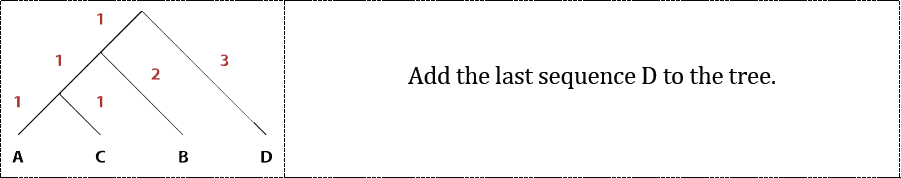
\includegraphics[width=0.9 \textwidth]{fig09/upgma_3.png}
\end{figure}

%
% Evaluation on how well fitted to the original distances
%
\subsubsection*{Evaluation on how well fitted to the original distances}
Several criteria are available to find the best-fitted tree for a given distance matrix, such as the Cavalli-Sforza and Edwards criterion:

\[
\sum_{i,j}{}(M_{i,j} - d_{i,j})^2
\]

where $M_{i,j}$ and $d_{i,j}$ are respectively the original and the calcualted pairwise distances.

%
% Example of the Cavalli-Sforza and Edwards criterion 
%
\subsubsection*{Example of the Cavalli-Sforza and Edwards criterion}

\begin{table}[H]
\centering
\begin{tabular}{lllllllll}
\multicolumn{4}{l}{Original}                                                                       &                       & \multicolumn{4}{l}{Reconstructed}                                                                 \\ \cline{1-4} \cline{6-9} 
\multicolumn{1}{|l|}{}  & \multicolumn{1}{l|}{B} & \multicolumn{1}{l|}{C} & \multicolumn{1}{l|}{D} & \multicolumn{1}{l|}{} & \multicolumn{1}{l|}{}  & \multicolumn{1}{l|}{B} & \multicolumn{1}{l|}{C} & \multicolumn{1}{l|}{D} \\ \cline{1-4} \cline{6-9} 
\multicolumn{1}{|l|}{A} & \multicolumn{1}{l|}{4} & \multicolumn{1}{l|}{2} & \multicolumn{1}{l|}{5} & \multicolumn{1}{l|}{} & \multicolumn{1}{l|}{A} & \multicolumn{1}{l|}{4} & \multicolumn{1}{l|}{2} & \multicolumn{1}{l|}{6} \\ \cline{1-4} \cline{6-9} 
\multicolumn{1}{|l|}{B} & \multicolumn{1}{l|}{}  & \multicolumn{1}{l|}{4} & \multicolumn{1}{l|}{8} & \multicolumn{1}{l|}{} & \multicolumn{1}{l|}{B} & \multicolumn{1}{l|}{}  & \multicolumn{1}{l|}{4} & \multicolumn{1}{l|}{6} \\ \cline{1-4} \cline{6-9} 
\multicolumn{1}{|l|}{C} & \multicolumn{1}{l|}{}  & \multicolumn{1}{l|}{}  & \multicolumn{1}{l|}{5} & \multicolumn{1}{l|}{} & \multicolumn{1}{l|}{C} & \multicolumn{1}{l|}{}  & \multicolumn{1}{l|}{}  & \multicolumn{1}{l|}{6} \\ \cline{1-4} \cline{6-9} 
\end{tabular}
\end{table}

\[
\sum_{i,j}{}(M_{i,j} - d_{i,j})^2 = 2((5-6)^2 + (8-6)^2 + (5-6)^2) =12
\]

%
% WPGMA
%
\subsubsection*{WPGMA}
WPGMA is a weighted version of PGMA.

\[
D_{w,x}=\dfrac{D_{u,x} + D_{\upsilon,x}}{2}
\]

%
% Neighbor-joining (NJ) method
%
\subsubsection*{Neighbor-joining (NJ) method}
It stats with the initial tree and then select two seqences which results in the smallest sum of edge lengths. It continues until there are no sequences to join. Unlike UPGMA, it does not require a constant evolutionary rate.

\begin{figure}[H]
  \centering
      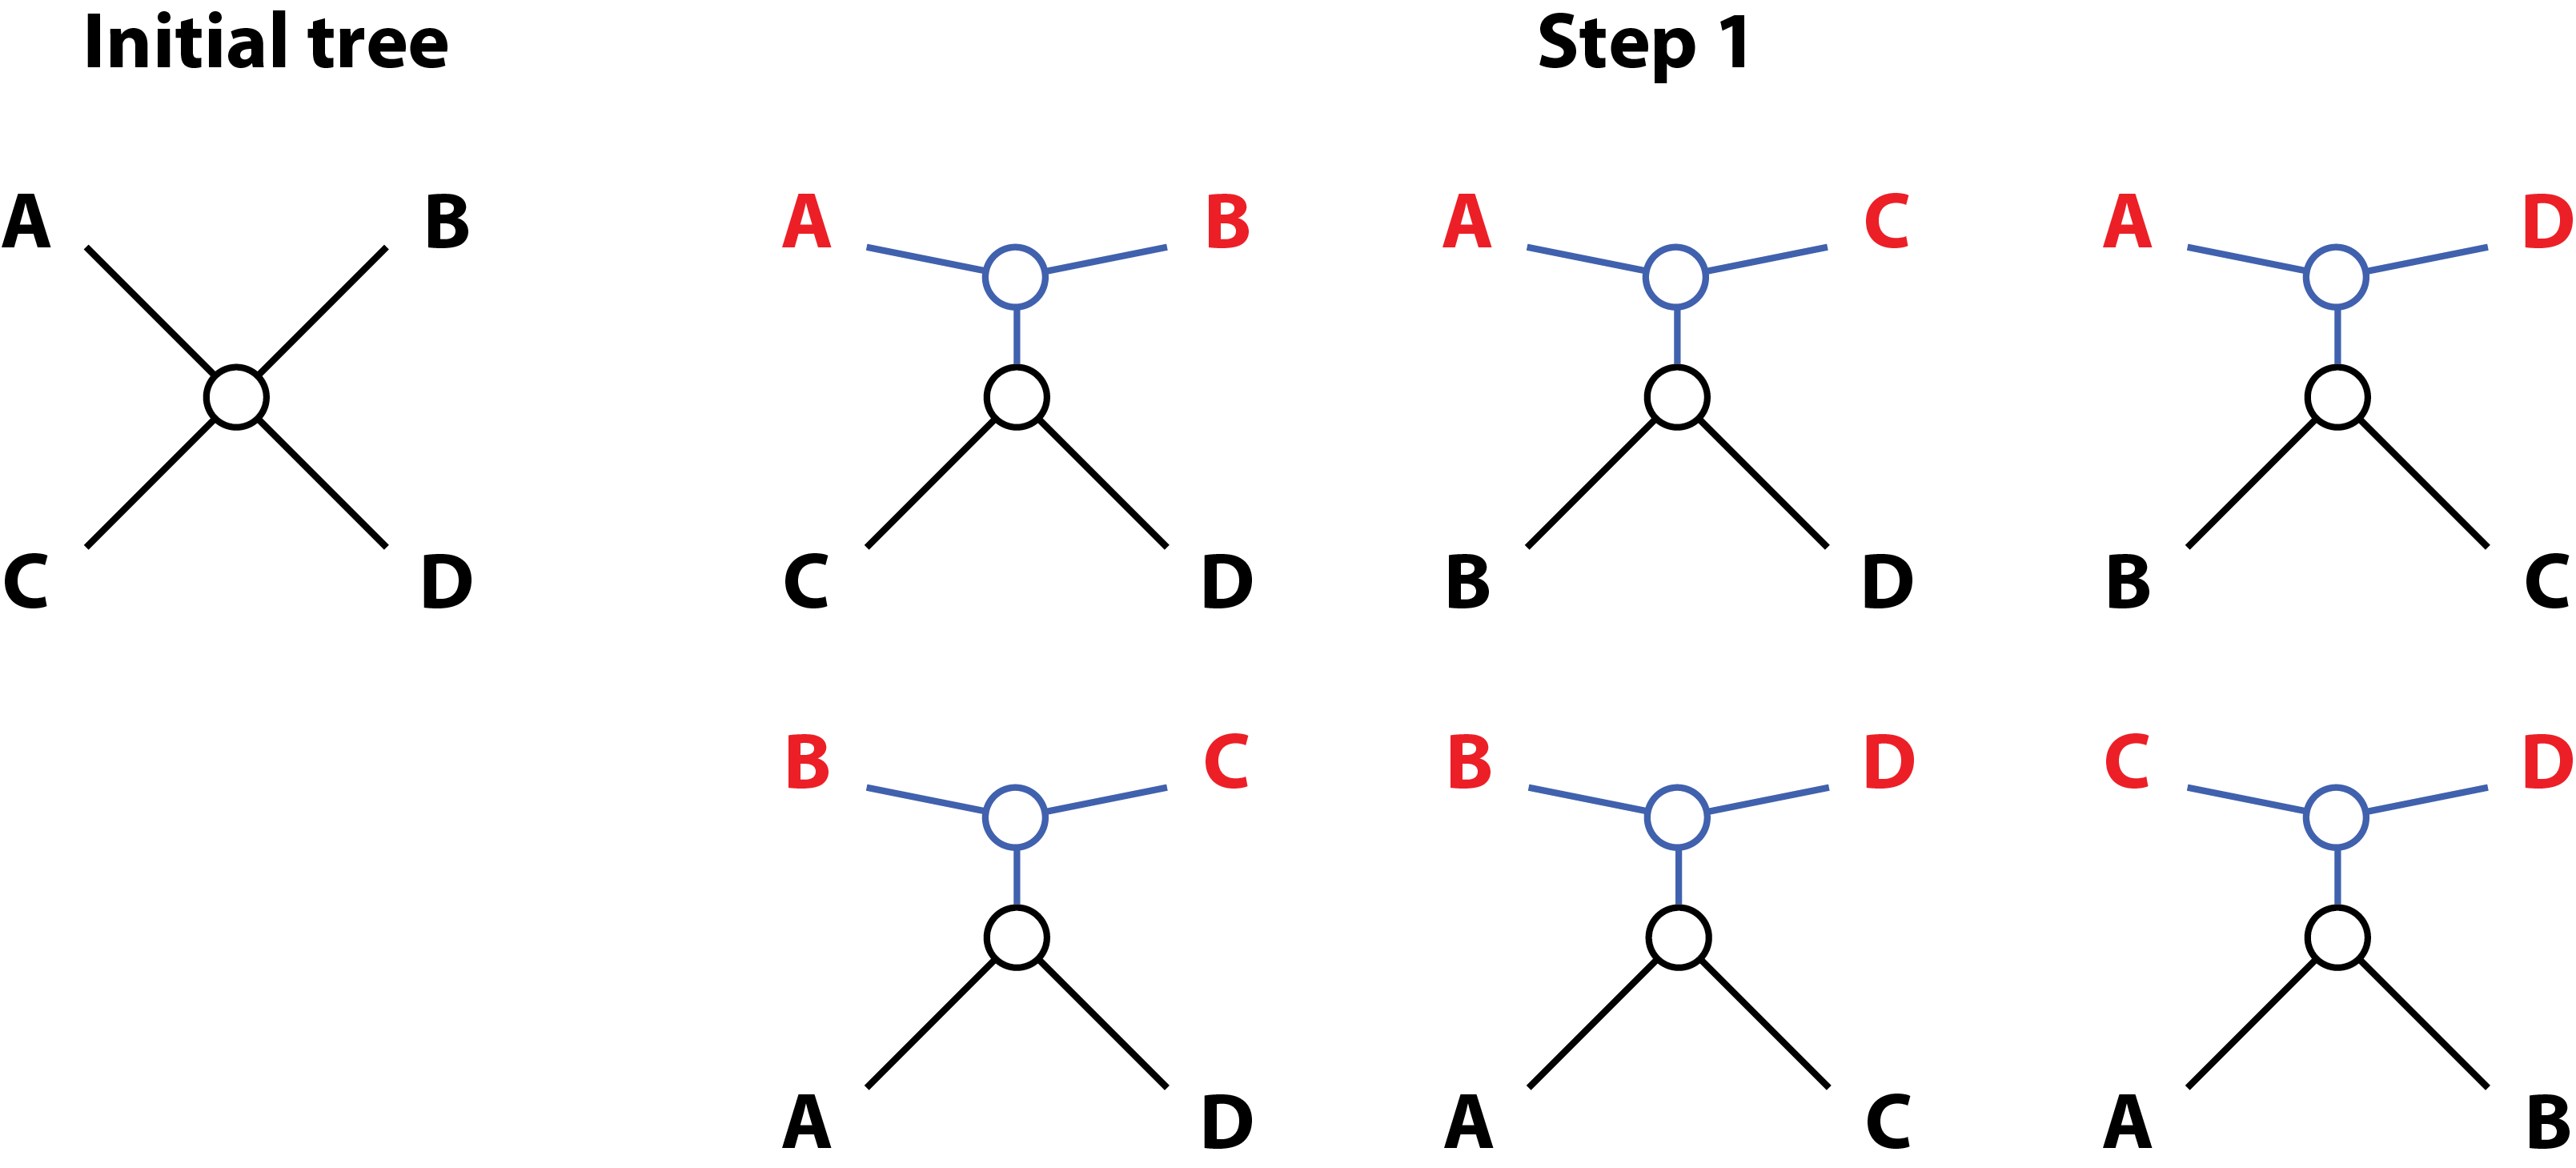
\includegraphics[width=0.75 \textwidth]{fig09/neighbor_joining.png}
  \caption{All possible combinations of adding one node the four sequences}
\end{figure}

%
% Exercise \thesection.2
%
\subsubsection*{Exercise \thesection.2}
\begin{enumerate}
\item Reconstruct a phylogenetic tree by using UPGMA and the following pre-calculated distances.
\begin{table}[H]
\centering
\begin{tabular}{|l|l|l|}
\hline
     & B & C \\ \hline
A  & 2 & 3 \\ \hline
B   &   & 5 \\ \hline
\end{tabular}
\end{table}

\item Create the distance matrix of the reconstructed tree. 
\begin{table}[H]
\centering
\begin{tabular}{|l|l|l|}
\hline
     & B & C \\ \hline
A  &  &  \\ \hline
B   &   &  \\ \hline
\end{tabular}
\end{table}

\item Calculated the Cavalli-Sforza and Edwards criterion.

\end{enumerate}

\bigskip 

%\end{document}
